% -----------------------------------------------------------------------------
% !Mode:: "TeX:Hard:CP1252"
% PDFLaTeX this document and view or print it from Acrobat Reader!
% -----------------------------------------------------------------------------
% Preamble Starts here:
% -----------------------------------------------------------------------------

\documentclass{article}
\usepackage[ansinew]{inputenc} % ASCII (Western Windows CP1252)
\usepackage{graphicx}
% This package converts eps figures to pdf during the compilation with PDFLaTeX.
% Converting images at this stage is a waste of CPU but (if for some reason)
% you cannot provide pdf or png alternatives this is a brute force solution
% to import eps graphics into pdf documents...
% \usepackage{epstopdf}
\usepackage{color}
\usepackage[colorlinks]{hyperref}
% \Add{} and \Del{} Corrections and \Mark{}
\usepackage[active,new,noold,marker]{xrcs}

% WinEdt's Bullets --------------------------------------------------------
% Allow WinEdt's Bullets (placeholders) in TeX Files!
% The bullets (eg. in automatically generated tables)
% should be replaced by actual data. In WinEdt you can
% use Ctrl+Space (Tools menu -> Next Bullet) to navigate
% through bullets and replace them with "real" entries...
\catcode`\=13
\def{$\bowtie$}

% EURO --------------------------------------------------------------------
%\usepackage{textcomp} %\texteuro: poor design
%
% Get it from CTAN if it is not included in your TeX distribution
%\usepackage{europs}
%\DeclareInputText{128}{\EUR} % ANSI code for euro: �
%     \EURhv     selects EuroSans
%     \EURtm     selects EuroSerif
%     \EURcr     selects EuroMono
%     \EUR       selects one of the three above, depending on the current
%                context
%
%     \EURofc    selects EuroSans Regular independent of context
%                N.B.: This is the only "official" Euro symbol. If you
%                      want to conform with the rules of the EU (or
%                      whoever), you may only use this symbol.
%
% HINT: Use MiKTeX's Package Manager to install eurosym package!
\usepackage{textcomp} % required for \texteuro
\usepackage{eurosym}  % required for \euro
\DeclareInputText{128}{\euro} % ANSI code for euro: � \usepackage{eurosym}
\DeclareInputText{165}{\yen}  % ANSI code for yen:  � \usepackage{amssymb}

\usepackage{lscape} %landscape pages support
% Your previewer may not support rotated boxes...

% -----------------------------------------------------------------------------
% More TeX Samples and Documentation
% -----------------------------------------------------------------------------
%  For more interesting examples check the MiKTeX's "...Doc\MiKTeX"
%  folder. You'll find examples of graphic inclusion, hyper-references,
%  and the use of colors....
%
%  In particular, take a look at:
%
%    epsdemo.tex
%    bmpdemo.tex
%    hyperdemo.tex
%    colordemo.tex
%
%  You'll find out which formats are supported by different conversion
%  utilities, etc...
%
%  Finally, while you are there don't forget to read the MiKTeX.*
%  manual (in your favorite format)!
% -----------------------------------------------------------------------------
% Document Starts here:
% -----------------------------------------------------------------------------

\begin{document}

\section{Graphics Inclusion}

\emph{Graphic inclusion in TeX documents is not a WinEdt-related issue. You
should consult the documentation that comes with your TeX System (eg.
graphicx package). Below are a few examples that show that it can be done! It
works with my (default) version of MiKTeX 2.9. However, these examples come
with no guarantee and no support from WinEdt Team. If you are experiencing a
problem with these images then the problem has nothing to do with WinEdt but
rather than your TeX System or Ghostscript...}

\bigskip

\noindent\textbf{Example 1:} WinEdt.eps (70 KB) (jpeg2ps wrapper). Bitmap
graphics does not scale well. Quality is further reduced when jpeg file is
formatted in order to reduce its size.

\medskip

\noindent\emph{PDFLaTeX uses a WinEdt.png (53 KB) when present. It gives
superior result compared to dvi2pdf or ps2pdf which (when properly
configured) use Ghostscript to convert eps images to pdf during the
compilation.}

\bigskip

\begin{center}
  
\includegraphics[width=2.5in]{Images/WinEdt}
\end{center}

\bigskip

\noindent \emph{Preparing two sets of graphic files (eps for dvi and ps
formats and pdf, png or jpg for pdf files) makes PDFTeX-ing easier! jpeg is a
good format for pictures (non-vector graphics) like the ones below:}

\bigskip

\begin{center}
  \begin{tabular}{cc}
    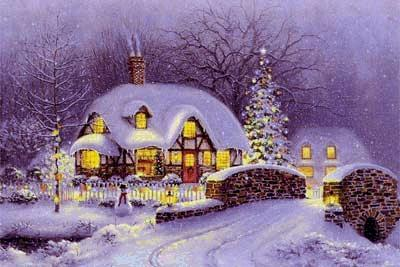
\includegraphics[width=2.15in]{Images/xmas} &
    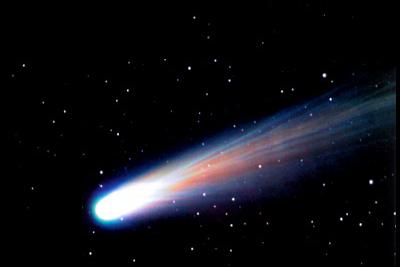
\includegraphics[width=2.15in]{Images/Comet}
  \end{tabular}
\end{center}

\bigskip
\goodbreak

\noindent \textbf{Example 2:}

\bigskip

\noindent The examples below are based on a ``proper'' eps file golpher.eps
(a vector graphics sample that comes with Ghostscript). The second instance
golpher1.eps represents the same wrapped image (jpeg2ps) after jpg was
compressed to a size (almost) comparable with the size of the original eps
file. PDFLaTeX uses png and jpg versions of images. You can compare the
quality (vector vs. bitmap graphics) depending on your favorite method of
compiling pdf files...

\medskip

\begin{verbatim}
    golfer.eps     (27 KB)
    golfer.png     (10 KB)
    golfer1.eps    (48 KB)
    golfer1.jpg    (37 KB)
\end{verbatim}

\medskip

\begin{center}
  \begin{tabular}{cc}
    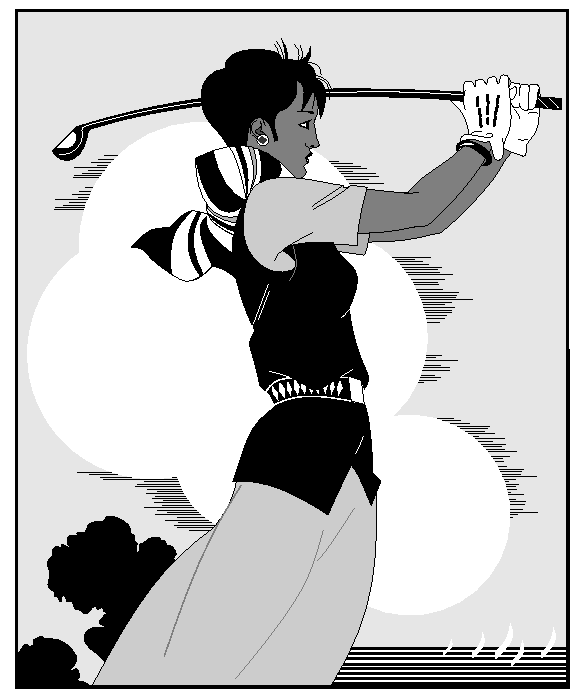
\includegraphics[width=2.22in]{Images/golfer} &
    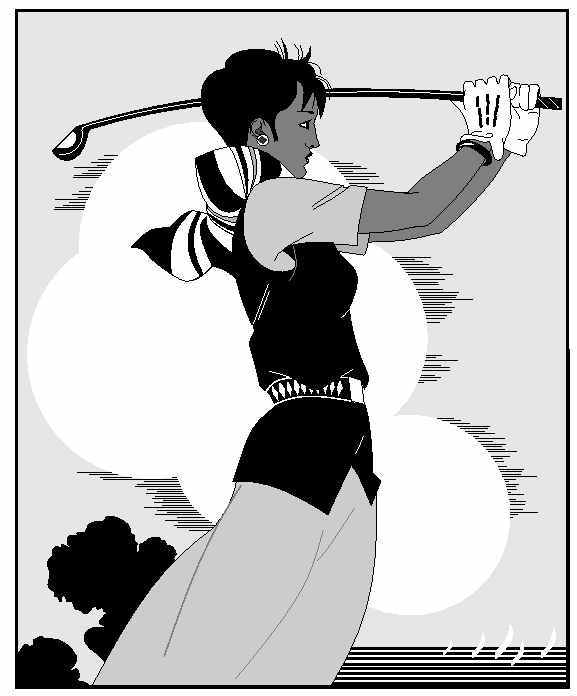
\includegraphics[width=2.22in]{Images/golfer1}
  \end{tabular}
\end{center}

\bigskip
\medskip

\noindent A similar example with TUG logo:

\bigskip

\begin{center}
  \begin{tabular}{cc}
    
\includegraphics[width=2.22in]{Images/TUG} &
    
\includegraphics[width=2.22in]{Images/TUG1}
  \end{tabular}
\end{center}

\newpage

% -----------------------------------------------------------------------------

\section{Color Package Example}

\emph{This section is ``borrowed'' from MiKTeX's Samples folder. You should
definitely consult more documentation and examples that come with your TeX
System...}

\bigskip

{\color{green} Text starts off in green \textcolor{red}{ a little red}
{\color{blue}nested blue text} returning to green}

\begin{enumerate}
  \item \textcolor[cmyk] {0,1,0,0}{magenta cmyk} black
  \item \color[gray]{0.5} \textcolor{blue}{predefined blue} gray text
\end{enumerate}

\definecolor{Light}{gray}{.80}
\definecolor{Dark}{gray}{.20}
\colorbox{red}{Black text on red background}
\par\colorbox{Light}{%
  \textcolor{Dark}{Light background}}
\par\colorbox{Dark}{%
  \textcolor{white}{Dark background}}

\fcolorbox{red}{blue}{Black text,
      blue background, red frame}

\fcolorbox{red}{blue}{\color{white}%
  White text, blue background, red frame}

\bigskip

\bigskip

\noindent \emph{This is how it is done:}

\medskip

\begin{verbatim}
  \usepackage{color}

    ...

      \begin{enumerate}
      \item \textcolor[cmyk]
         {0,1,0,0}{magenta cmyk}  black
      \item \color[gray]{0.5}
        \textcolor{blue}{predefined blue}
         gray text
      \end{enumerate}

      \definecolor{Light}{gray}{.80}
      \definecolor{Dark}{gray}{.20}
      \colorbox{red}{Black text on red background}
      \par\colorbox{Light}{%
        \textcolor{Dark}{Light background}}
      \par\colorbox{Dark}{%
        \textcolor{white}{Dark background}}

      \fcolorbox{red}{blue}{Black text,
            blue background, red frame}

      \fcolorbox{red}{blue}{\color{white}%
        White text, blue background, red frame}
\end{verbatim}

\newpage

% -----------------------------------------------------------------------------

\section{Rotated tables examples}

These are rotated tables:

\bigskip

\begin{center}

\rotatebox{0}{
\begin{tabular}{|c|c|c|c|c|c|}
  % after \\: \hline or \cline{col1-col2} \cline{col3-col4} ...
  xx & yy & zz & a & b & c \\
  xx & yy & zz & a & b & c \\
  xx & yy & zz & a & b & c \\
\end{tabular}
}

\bigskip

\rotatebox{30}{
\begin{tabular}{|c|c|c|c|c|c|}
  % after \\: \hline or \cline{col1-col2} \cline{col3-col4} ...
  xx & yy & zz & a & b & c \\
  xx & yy & zz & a & b & c \\
  xx & yy & zz & a & b & c \\
\end{tabular}
}

\bigskip

\rotatebox{45}{
\begin{tabular}{|c|c|c|c|c|c|}
  % after \\: \hline or \cline{col1-col2} \cline{col3-col4} ...
  xx & yy & zz & a & b & c \\
  xx & yy & zz & a & b & c \\
  xx & yy & zz & a & b & c \\
\end{tabular}
}

\bigskip

\rotatebox{90}{
\begin{tabular}{|c|c|c|c|c|c|}
  % after \\: \hline or \cline{col1-col2} \cline{col3-col4} ...
  xx & yy & zz & a & b & c \\
  xx & yy & zz & a & b & c \\
  xx & yy & zz & a & b & c \\
\end{tabular}
}

\bigskip

\rotatebox{180}{
\begin{tabular}{|c|c|c|c|c|c|}
  % after \\: \hline or \cline{col1-col2} \cline{col3-col4} ...
  xx & yy & zz & a & b & c \\
  xx & yy & zz & a & b & c \\
  xx & yy & zz & a & b & c \\
\end{tabular}
}

\end{center}

% -----------------------------------------------------------------------------

\newpage

\landscape

\begin{center}

\textbf{\large This page is displayed in landscape mode...}

\vskip 1cm

\begin{tabular}{|c|c|c|c|c|c|}
  % after \\: \hline or \cline{col1-col2} \cline{col3-col4} ...
  xx & yy & zz & a & b & c \\
  xx & yy & zz & a & b & c \\
  xx & yy & zz & a & b & c \\
  xx & yy & zz & a & b & c \\
  xx & yy & zz & a & b & c \\
  xx & yy & zz & a & b & c \\
  xx & yy & zz & a & b & c \\
  xx & yy & zz & a & b & c \\
  xx & yy & zz & a & b & c \\
  xx & yy & zz & a & b & c \\
  xx & yy & zz & a & b & c \\
\end{tabular}

\vskip 2cm

\emph{\textbf{Rotated Table}}

\end{center}

\endlandscape

\newpage

% -----------------------------------------------------------------------------

\section{Presentations in \LaTeX}

Presentation packages and software that can be used with \LaTeX\ is not a
WinEdt-related topic. However, since we get frequently asked about such
things we posted a question to WinEdt's Mailing List and the response was
overwhelming.

\bigskip

Most users were of the opinion that \emph{beamer} is currently the best when
it comes to ease of use and the quality of the output. Alternatives have also
been mentioned. Below is the summary of the relevant links:

\begin{itemize}
  \item \url{http://latex-beamer.sourceforge.net/}
  \item \url{http://texpower.sourceforge.net/}
  \item \url{http://www.utopiatype.com.au/}
  \item \url{http://tug.org/applications/Seminar/}
  \item
      \url{http://www-sp.iti.informatik.tu-darmstadt.de/software/ppower4}
\end{itemize}

\bigskip

You can use MiKTeX's Package Manager to install \emph{beamer}. In MiKTeX's
Doc folder you'll find documentation and examples that can be used to help
you start working on your presentations. Some users mentioned that they had
to upgrade their MiKTeX in order to be able to compile these examples which
rely on up-to-date packages. If you encounter any such problems you may have
to do the same...

\bigskip

An often cited reference summarizing the available \LaTeX-related
presentation packages is:

\begin{itemize}
  \item \url{http://www.miwie.org/presentations/presentations.html}
\end{itemize}

\bigskip

You should visit the site to see what is currently available. Many packages
are under development and the above links reflect the situation at the end of
2004. Things may change in the future and so can the contents of any of the
sites listed on this page (this is outside our control)...

\bigskip
\bigskip

\noindent \emph{Again:} do not expect any support from the WinEdt Team when
it comes to purely \LaTeX\ issues (like the one concerning presentations)...

\bigskip

\noindent You can find everything about \TeX\ and \LaTeX\ on:
\url{http://www.tug.org}...

\newpage

% -----------------------------------------------------------------------------

\section{A Simple Revision Control System (RCS)}

\noindent On \href{http://www.winedt.org}{www.winedt.org} you'll find a link
to the page that describes how to use RCS or CS-RCS with WinEdt. RCS
(Revision Control System) is a proper way to deal with revisions...

However, simple revisions or corrections done by the copy editor and intended
for the authors can be handled in a much simpler manner. WinEdt provides a
sample LaTeX package \texttt{xrcs.sty} that can be used for such editing. The
package defines two macros \verb"\RCSAdd{...}" and \verb"\RCSDel{...}". These
two macros can be used to mark simple additions and deletions, respectively.
In WinEdt the environments are colored in blue and red (as defined in the
Switches section of the Options interface). Depending on the options the
compiled document can contain additions and/or deletions (in color or plain
text).

Furthermore, the package also provides a tag \verb"\RCSMark{...}" which can
be used to mark the argument with a yellow marker and \verb"\RCSRem{...}"
which can be used to include remarks. All four RCS tags are defined as
switches in WinEdt's default highlighting scheme for TeX mode.

\bigskip

\noindent The \texttt{xrcs.sty} package provides the following options (with
the default values displayed in red):

\begin{center}
  \begin{tabular}{|l|l|}
    \hline
    \texttt{active}              &  \texttt{\color{red}{inactive}}  \\
    \texttt{\color{red}{marker}} &  \texttt{nomarker}               \\
    \texttt{remarks}             &  \texttt{\color{red}{noremarks}} \\
    \texttt{\color{red}{new}}    &  \texttt{nonew}                  \\
    \texttt{old}                 &  \texttt{\color{red}{noold}}     \\
    \hline
  \end{tabular}
\end{center}

\noindent Examples of usage:

\begin{verbatim}
  \usepackage[active,new,old,remarks,marker]{xrcs}
  \usepackage[active]{xrcs} % Only Additions- in blue colors
  \usepackagep[active,old,nonew]{xrcs} % Only old text - in red
  \usepackage[nomarker}{xrcs} % Only Additions: final version
\end{verbatim}

\noindent In your preamble you have to also include the color package:

\begin{verbatim}
  \usepackage{color}
\end{verbatim}

\noindent Text example:

\begin{verbatim}
  \RCSMark{IMPORTANT:} WinEdt's \RCSDel{menu}\RCSRem{use capitals!}
  \RCSAdd{Menu} should be thought of as an ``Action List''...
\end{verbatim}

\noindent with \verb"\usepackage[active,new,noold,marker]{xrcs}" is processed
as:

\bigskip

\RCSMark{IMPORTANT:} WinEdt's \RCSDel{menu}\RCSRem{use capitals!}
\RCSAdd{Menu} should be thought of as an ``Action List''...

\newpage

Beside the highlighting definitions for switches \verb"\RCS*{...}" WinEdt
also has a popup menu \texttt{Edt RCS} containing some commands that can make
the revisions easier. This popup menu is displayed in response to the
\texttt{Alt+R} keystroke. The properties of the popup can be adjusted through
the Options interface (Popup Menus)...

WinEdt Team does not provide support for the package \texttt{xrcs.sty}. Feel
free to make changes and improvements... The file is by default located in:

\begin{verbatim}
 %b\Samples\Examples\xrcs.sty
\end{verbatim}

\begin{verbatim}
% -------------------------------------------------------------
% File: xrcs.sty
%
% A (very) simple Revision Control System for LaTeX2e/WinEdt
% *************************************************************
\NeedsTeXFormat{LaTeX2e}
\ProvidesPackage{xrcs}[2005/01/30 v0.002 RCS]
\RequirePackage{color}
\newif\ifMarker \Markertrue
\newif\ifRemarks\Remarkstrue
\newif\ifAddDel \AddDeltrue
\newif\ifAddNew \AddNewtrue
\newif\ifAddOld \AddOldfalse
\DeclareOption{active}{\AddDeltrue}
\DeclareOption{inactive}{\AddDelfalse}
\DeclareOption{marker}{\Markertrue}
\DeclareOption{nomarker}{\Markerfalse}
\DeclareOption{remarks}{\Remarkstrue}
\DeclareOption{noremarks}{\Remarksfalse}
\DeclareOption{new}{\AddNewtrue}
\DeclareOption{nonew}{\AddNewfalse}
\DeclareOption{old}{\AddOldtrue}
\DeclareOption{noold}{\AddOldfalse}
\ExecuteOptions{inactive,noold,noremarks,new,marker}
\ProcessOptions
% -------------------------------------------------------------
\def\RCSMark#1{\ifMarker{\colorbox{yellow}{#1}}\else#1\fi}
\def\RCSRem#1{\ifRemarks{\textsf{#1}}\fi}
\def\RCSDel#1{\ifAddOld\ifAddDel{\color{red}#1}\else#1\fi\fi}
\def\RCSAdd#1{\ifAddNew\ifAddDel{\color{blue}#1}\else#1\fi\fi}
%--------------------------------------------------------------
\end{verbatim}


\emph{Once again, this is a very simplified revision system; it is somewhat
primitive and it is lacking all the features available in proper RCS...
However, it may be of some interest since it is very simple to use: in any
text editor it is easy to search for} \verb"\RCS"...

\newpage

% -----------------------------------------------------------------------------

\section{Useful \TeX-ing Hints}

\noindent \emph{Check the source code of this document in WinEdt. Pay
attention to comments included in the preamble...}

\bigskip

\noindent For author-year references use:

\begin{verbatim}
    \usepackage{natbib}
\end{verbatim}

\bigskip

\noindent Specify bibliography database in a different folder:

\begin{verbatim}
    \bibliography{Biblio/articles.bib}
\end{verbatim}

Note that you have to specify the path in UNIX-style (using forward instead
of backward slash as folder separator). Avoid spaces in filenames (some TeX
accessories may not work properly with spaces in filename specification).

\emph{Most TeX Systems allow you to place your bib files in a separate folder
on your localtexmf tree. For details consult the documentation that comes
with your TeX System. MiKTeX users can create a bibtex folder in their
localtexmf tree, place their bib files there, and refresh the FNDB in
MiKTeX's Options interface.}

\bigskip

\noindent For fancy pdf files use:

\begin{verbatim}
    \usepackage{hyperref}
    \hypersetup{
       pdftitle={Shown in AR File Information},
       pdfstartview=FitH,   % Fit the page horizontally
       bookmarks=true,      % Open Bookmarks in AR
    }
    % more options can be found in
    % TEXMF/doc/latex/hyperref/manual.pdf
\end{verbatim}

\bigskip

\noindent To manually correct hyphenation of a word that was not properly
handled by \TeX\ (eg. Weltauffassung) put the following in the preamble:

\begin{verbatim}
    \hyphenation{Welt-auf-fas-sung}
\end{verbatim}

\bigskip

\noindent To prevent long titles in your table of contents (generated by
\LaTeX) use alternative short title:

\begin{verbatim}
    \section[Short Title for TOC]{Long long long title}
\end{verbatim}

\bigskip

\noindent \emph{You can find everything about \TeX\ and \LaTeX\ on:}
\href{http://www.tug.org}{TUG}...

\end{document}

% -----------------------------------------------------------------------------
